\documentclass[11pt]{article}

\usepackage[margin=1.15in]{geometry}
 \usepackage{vwcol}

\usepackage[T1]{fontenc}\usepackage[T1]{fontenc}
\usepackage[latin1]{inputenc}

\usepackage{lmodern}
\usepackage{comment}
\usepackage[scaled=0.95]{inconsolata}
\usepackage{booktabs}

\usepackage{graphicx}
\usepackage{floatrow} % for horizontal captions
\usepackage{amsmath,amsfonts,amssymb}
\usepackage[capitalize]{cleveref}
\usepackage{icomma}
\usepackage{parskip}

\usepackage{enumitem}

\usepackage{xcolor}

\graphicspath{{figures/}}

\usepackage{fancyhdr}
\pagestyle{fancy}
\fancyhf{} % sets both header and footer to nothing
\lhead{16.90 Computational Methods in Aerospace Engineering}
\rhead{Spring 2017}
\setlength{\headheight}{14pt}
%\renewcommand{\headrulewidth}{0pt}

\begin{document}
\begin{center}
\Large\textbf{Project 3: Probabilistic Simulation of an Airdrop Payload}\\[1em]
\normalsize Final report due Friday, May 12 at 5:00pm (outside of 37-312)
\end{center}
\hrulefill\\[1em]
\textbf{Note:} \textit{Projects are meant to be open-ended and to
  allow some flexibility and creativity. Therefore it is important
  for you to show all relevant steps, numerical plots, and
  justifications for the choices made in your work.}

\hrulefill

\section{Background}
In peacekeeping operations or humanitarian aid situations, food and
medical supplies are often airdropped from aircraft to resupply
otherwise inaccessible personnel on the ground. In this project, we
will analyze the delivery of a payload involving parachutes that are
designed to slow down the payload as much as possible to ensure that it impacts the ground with minimal force. This type of airdrop is used for delicate equipment and larger items such as vehicles.

In this project you will use Monte Carlo analysis to determine whether an airdrop payload design will satisfy the mission criteria.

\subsection{System dynamics}
Provided for you is the function \texttt{payload\_sim.m} that calculates the trajectory of the payload dropped from an aircraft by solving a system of ODEs. The inputs to this function are:
\begin{itemize}
  \item $u(0)=[x(0), y(0), v_x(0), v_y(0)]$, horizontal and vertical displacements and velocities.
  \item $m$, the mass of the payload in kilograms.
  \item $r$, the radius of the payload in meters.
  \item $C_d$, the coefficient of drag for the payload.
  \item $w_x$, the horizontal wind speed in m/s.
  \item $t_\text{free}$, the time that the payload is in free-fall before the parachute is opened.
  \item $t_\text{open}$, the time in seconds that it takes for the parachute to open to its full size.
\end{itemize}
After being released from the aircraft, the payload enters free-fall
for $t_\text{free}$ seconds, at which time the parachute begins is
deployed. The parachute takes $t_\text{open}$ seconds to open
fully. There is a maximum parachute drag force of $F_\text{max}=300\,\text{N}$, that when exceeded will result in the parachute becoming detached from the payload.

The code computes the trajectory of the payload as a function of time by numerically integrating a system of ODEs until $y(t)=0$. The function returns two arrays: the first is the time at each simulated timestep, and the second is the state of the payload at each timestep, i.e.,
\[ \mathbf{t}=\begin{bmatrix}0\\\vdots\\t_f\end{bmatrix},\quad
\mathbf{u}=\begin{bmatrix} x(0) & y(0) & v_x(0) & v_y(0) & \texttt{detached}(0) \\
\vdots &\vdots &\vdots &\vdots &\vdots \\
x(t_f) & y(t_f)=0 & v_x(t_f) & v_y(t_f) & \texttt{detached}(t_f)\end{bmatrix}\]
where $\texttt{detached}(t)\in\{0,1\}$ indicates if the parachute is attached to the payload at time $t$. The simulation runs until the payload hits the ground, so the last row of $\mathbf{u}$ corresponds to the exact moment of impact where $y(t_f)=0$. This fact will be useful when classifying the outcome of each simulated trajectory.

A reference trajectory is plotted in \cref{fig:trajectory}, where the parachute opens successfully and the payload impacts the ground with a low velocity. On the other hand, if we reduce the parachute opening time from $t_\text{open}=5$ to $t_\text{open}=2$ seconds, then the drag force on the parachute exceeds $F_\text{max}$, causing the parachute to become detached and the payload to impact the ground at an unacceptably high velocity; see \cref{fig:trajectory-torn}.
\begin{figure}[H]
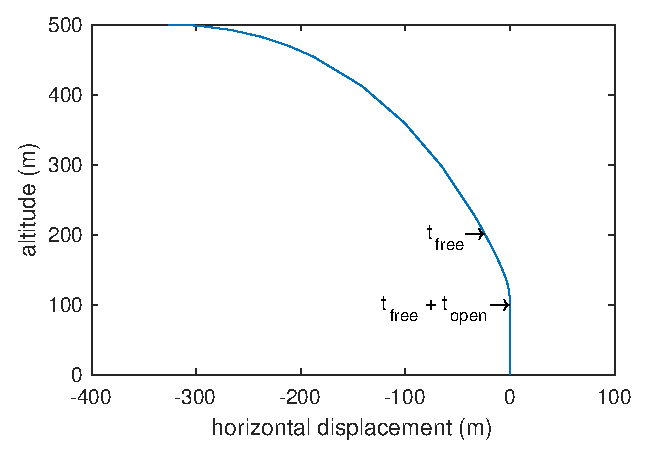
\includegraphics[width=0.48\textwidth]{figures/trajectory.eps}
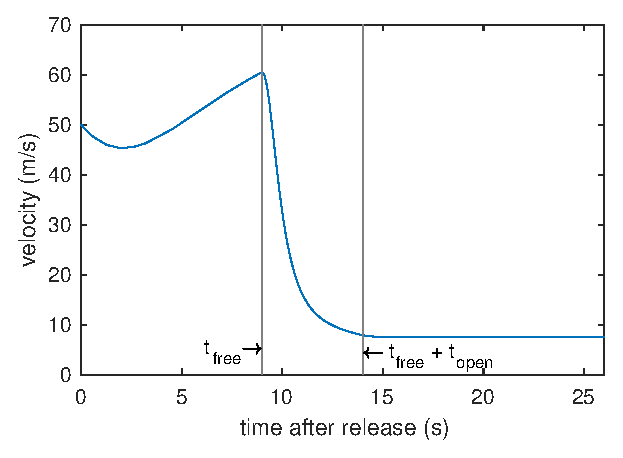
\includegraphics[width=0.46\textwidth]{figures/velocity.eps}
\hspace{0.07\textwidth}
\caption{Payload trajectory simulated using nominal parameter values. Notice that the payload reaches a safe terminal velocity soon after the parachute is fully open.}
\label{fig:trajectory}
\end{figure}
\begin{figure}[H]
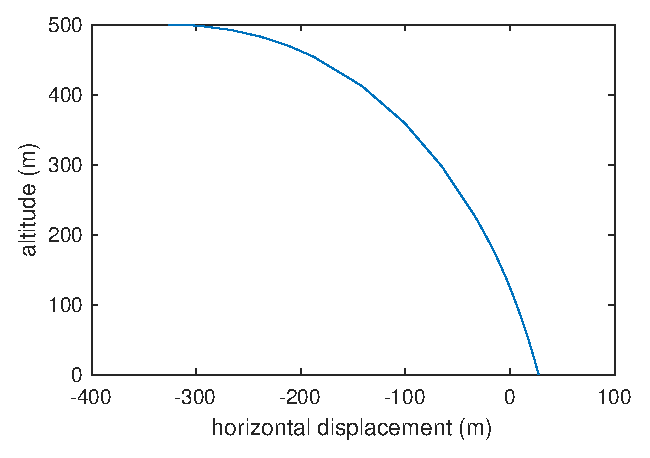
\includegraphics[width=0.48\textwidth]{figures/trajectory_torn.eps}
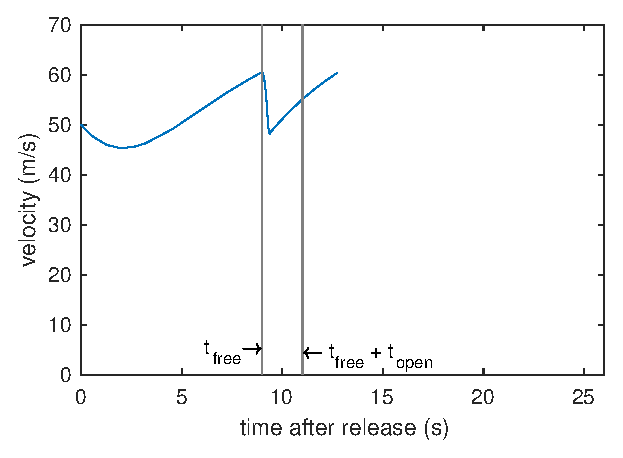
\includegraphics[width=0.46\textwidth]{figures/velocity_torn.eps}
\hfill
\caption{Payload trajectory simulated using a shorter parachute opening time $t_\text{open}=2\,\text{s}$, where the force on the parachute is too large and the parachute is torn off soon after it is deployed, which results in the payload impacting the ground at an unsafe velocity. }
\label{fig:trajectory-torn}
\end{figure}

\subsection{Mission criteria}
The payload must land intact within the designated area $x(t_f)\in[-50\,\text{m}, 50\,\text{m}]$ with greater than 75\% probability to be considered a success.

\subsection{Input uncertainty}
We will assume that each of the variable inputs to the payload simulation code are uncertain and can be modeled with either a normal, log-normal, or triangular distribution. The distribution type and parameters for each uncertain variable/parameter are given in \cref{tbl:distributions}. For the triangular distributions, Min, Mode, and Max denote the minimum, most-probable, and maximum values respectively. For the normal and log-normal distributions, $\mu$ is the mean value and $\sigma^2$ is the variance. Note, if $Z\sim\mathcal{N}(0, 1)$, then $X=\exp(\mu+\sigma Z)$ is log-normally distributed, i.e., $X\sim\ln\mathcal{N}(\mu, \sigma^2)$.

\begin{table}[H]
  \begin{tabular}{cccccccc}\toprule
  Variables & Units & Distribution type & $\mu$ & $\sigma^2$ & Min & Mode & Max \\ \midrule
  $x(0)$ & m & normal & $-340$ & $(3.0)^2$ & -- & -- & -- \\
  $y(0)$ &m & normal & 500 & $(3.0)^2$ & -- & -- & -- \\
  $v_x(0)$ & m/s & normal & 50 & $(0.5)^2$ & -- & -- & -- \\
  $v_y(0)$ & m/s & normal & 0 & $(0.5)^2$ & -- & -- & -- \\\midrule
  $m$ &kg & triangular & -- & -- & 4.00 & 6.00 & 9.00 \\
  $r$ &m & triangular & -- & -- & 0.09 & 0.10 & 0.11 \\
  $C_d$ & &triangular & -- & -- & 0.45 & 0.50 & 0.60 \\
  $t_\text{free}$ & s & triangular & -- & -- & 8.95 & 9.00 & 9.05 \\
  $t_\text{open}$ & s & log-normal & 1.65 & $(0.15)^2$ & -- & -- & -- \\\midrule
  $w_x$ & m/s & normal & 0 & $(2.0)^2$ & -- & -- & -- \\\bottomrule
  \end{tabular}
  \caption{Distribution type and parameters for uncertain inputs}
  \label{tbl:distributions}
\end{table}

\subsection{Survival model}
Instead of modeling whether a payload survives impact by specifying a hard threshold on $v_f=|\vec{v}(t_f)|$, we specify the following survival function:
\begin{align*}
  S(v_f) = \frac{1}{2}-\frac{1}{2}\text{erf}\biggl(\frac{\log v_f-\mu}{\sqrt{2}\sigma}\biggr),\quad \mu=2.3,\quad \sigma=0.15,
\end{align*}
where $\mu$ and $\sigma$ were chosen so that there is a $\sim$99\% chance of survival at 7\,m/s and a $\sim$50\% chance of survival at 10\,m/s. The survival function is plotted in \cref{fig:survival}.
For the purpose of of Monte Carlo analysis, you can determine whether the payload survives impact for each simulated trajectory by checking if a standard uniform random variable $U\sim\mathcal{U}(0,1)$ is less than the survival probability given by $S(v_f)$.
\begin{figure}[H]
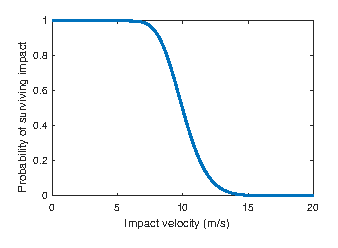
\includegraphics[width=0.48\textwidth]{figures/survival.eps}
\caption{Survival probability as a function of impact velocity}
\label{fig:survival}
\end{figure}

\section{Project Requirements}
\subsection{Estimation of the mission outcomes}
Implement a Monte Carlo analysis to determine the probability of the following outcomes:\\[0.5em]
\begin{minipage}{0.4\linewidth}
\begin{center}
  {\def\arraystretch{1.5}
  \begin{tabular}{r|c|c}
    & Inside & Outside \\ \hline
    Intact & \textbf{A} & \textbf{B} \\ \hline
    Destroyed & \textbf{C} & \textbf{D} \\
  \end{tabular}
  }
\end{center}
\end{minipage}
\begin{minipage}{0.6\linewidth}
\begin{enumerate}[label=\textbf{\Alph*:}]
  \item payload lands intact inside the designated area.
  \item payload lands intact outside the designated area.
  \item payload destroyed inside the designated area.
  \item payload destroyed outside the designated area.
\end{enumerate}
\end{minipage}

\begin{enumerate}
  \item Develop MATLAB scripts to implement the Monte Carlo analysis for this problem:
  \begin{itemize}
    \item Complete the function \texttt{logrand.m} to draw a sample from a log-normal distribution.
    \item Complete the function \texttt{trirand.m} to draw a sample from a triangular distribution.
    \item To draw samples from a normal distribution you can use the built-in \texttt{randn} function.

    \textbf{Note:} The only built-in MATLAB functions you should use to help generate your random samples are \texttt{rand} and \texttt{randn}.
    \item You will need to write a script to conduct the Monte Carlo simulation and perform the required analyses. Skeleton code for setting up the simulation is provided in \texttt{project3.m}. The function \texttt{payload\_sim()} will  be called inside your Monte Carlo loop but does not need to be modified.
  \end{itemize}
  \item Test that your sampling schemes are working by generating $N=1,000$ samples drawn from your input distributions. Plot a histogram of the inputs for the simulation. Do the inputs match what you expect? Also, run and plot 20 simulated trajectories (on a single axes) using samples from your input distributions.

  \item Estimate the probability of each of the four mission outcomes and identify the variance of each estimate. For estimating the probability of success (outcome \textbf{A}), choose a sample size $N$ so that your estimate is at least $\pm0.01$ at 99\% confidence.

  \item Plot histograms of the payload landing sites and impact velocities for payloads that surivived impact and those that did not. Discuss how the histograms vary for the different outcomes.

  \textbf{Note:} If you plan on overlaying multiple histograms on a single plot, make sure to use the same bin width so that the bin counts share the same vertical axis.
\end{enumerate}

\subsection{Design under uncertainty}
In the previous section, you will find that probability of success is lower than the desired probability of 75\%. Upon hearing this, the engineering team has proposed several design changes which they claim will increase the probability of success. Your job is to verify these claims by calculating the probability of success after implementing each proposed change individually, and the probability of success if all the proposed changes are implemented simultaneously.
\begin{enumerate}
  \item \textbf{Improved payload shock absorption} -- Increases the survival probability of payloads impacting at higher velocities so that $\mu=2.7$ in the survival function $S(v_f)$.
  \item \textbf{Stricter regulations on payload weight} -- Restricts extremely underweight and overweight payloads so that the input distribution becomes $m\sim\text{Triangular}(5, 6, 7)$.
  \item \textbf{Improved parachute deployment} -- Reduces the variance of parachute opening time so that the input distribution becomes $t_\text{open}\sim\ln\mathcal{N}(1.75, (0.1)^2)$.
\end{enumerate}
You should obtain $3+1$ estimates of the probability of success. Based on your results, what recommendation would you give the engineering team?

\subsection{Importance sampling}
Now, the payload is a proton torpedo, and the target area is a $2$-meter wide thermal exhaust port on a space station the size of a small moon. We retain the same parameter values and uncertainties, which describes the conditions when a pilot disables their targeting computer.
\begin{enumerate}
  \item  What is the probability of success? Repeat your Monte Carlo analysis (with the uncertainties in \cref{tbl:distributions}) at least 20 times and record the variance of your estimated probability of success with the new mission parameters.
\end{enumerate}
Since very few simulated trajectories will fall inside the target area, you will want to construct a biasing distribution by modifying the parameters of the input distributions and use importance sampling to reduce the variance in your estimate of the probability of success. A good rule-of-thumb for finding a biasing distribution is to have half of the samples from the biasing distribution result in a successful outcome.
\begin{enumerate}
\setcounter{enumi}{1}
\item Once you have found an appropriate biasing distribution, repeat your Monte Carlo analysis with the same number of samples as before. What is the variance of your importance sampling estimate?

\textbf{Note:} When computing the importance weights, you will need to know the probability density function for each type of distribution in the input uncertainties table, which you already know for the normal and triangular distributions. The density of a log-normal random variable $X\sim\ln\mathcal{N}(\mu, \sigma^2)$ is
\[ f_X(x)=\frac{1}{x\,\sigma\sqrt{2\pi}}\exp\biggl(-\frac{(\ln x-\mu)^2}{2\sigma^2}\biggr),\quad x>0.\]
\item\emph{(Optional)} Given that such an event was observed a long time ago, in a galaxy far, far away, is there reason to believe that there was something more than mere luck that allowed the pilot to make this shot?
\end{enumerate}

%\subsection{Sensitivity analysis (optional)}
%Use the provided \texttt{sensitivity\_analysis.m} function to perform global sensitivity analysis and to compute the main-effect sensitivities of your objective

\section{Report}
Turn in a concise, but professional, report that includes the following items:
\begin{itemize}
\item A description of your implementation of the numerical techniques, including any relevant derivations and choices for parameter values.
\end{itemize}
Please upload your report as a PDF file to Stellar in addition to submitting a hardcopy in class. If you are printing in black and white, please make sure your plot styles remain legible.

Also, please upload your commented code to Stellar in a standalone zip file.

\end{document}

